%%%%%%%%%%%%%%%%%%%%%%%%%%%%%%%%%%%%%%%%%%%%%%%%%%%%%%%%%%%%%%%%%%%%%%%%
\chapter{Results}\label{chap:results}
%%%%%%%%%%%%%%%%%%%%%%%%%%%%%%%%%%%%%%%%%%%%%%%%%%%%%%%%%%%%%%%%%%%%%%%%

% cosa metto qui? magari la parte delle metriche?

%%%%%%%%%%%%%%%%%%%%%%%%%%%%%%%%%%%%%%%%%%%%%%%%%%%%%%%%%%%%%%%%%%%%%%%%
\section{Metrics}
%%%%%%%%%%%%%%%%%%%%%%%%%%%%%%%%%%%%%%%%%%%%%%%%%%%%%%%%%%%%%%%%%%%%%%%%

Metrics give accurate measurements about how a process is functioning and provide a measure to suggest the improvements.
Developing and understanding standardized metrics is crucial to guide decision-making and prevent the need to make hasty decisions~\cite{austin2021need}.

As stated in \ref{sec:state-of-the-art}, skin detection is a two-class problem.
To evaluate a binary classifier, the ideal data (the ground truth) is compared to the predicted data given by the method.
In the case of skin detection, data is generally represented by binary masks.
The primitive metrics to define are the ones inside a confusion matrix, depicted in \autoref{fig:confmat}.
A \textbf{False Positive} is an error in binary classification in which a test result incorrectly indicates the presence of a condition such as a disease when the disease is not present.
A \textbf{False Negative} represents the opposite case: the test result incorrectly fails to indicate the presence of a condition when it is present.
These are the two kinds of errors in a binary test, in contrast to the two kinds of correct results (a \textbf{True Positive} and a \textbf{True Negative}).
It is important to note that the gravity of an error depends on the contest. %In the medical field, a False Negative may represent a bigger problem than a False Positive 
An example of different error seriousness is illustrated in \autoref{fig:bin-errors}.
In image segmentation, False Positives may represent a lesser gravity since a follow-up processing of the image could fix the issues, while the data of false negatives is lost.

\begin{figure}[h]
    \centering
    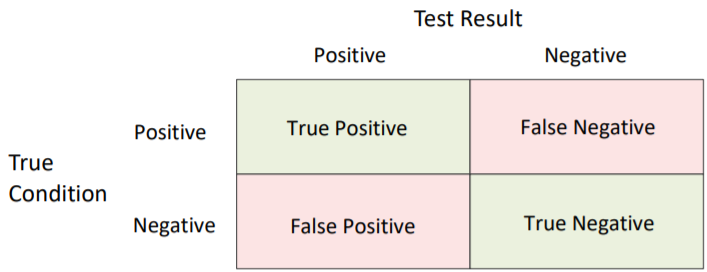
\includegraphics[width=0.7\linewidth]{images/results/confmat.png}
    \caption{A confusion matrix.}
    \label{fig:confmat}
\end{figure}

\begin{figure}[h]
    \centering
    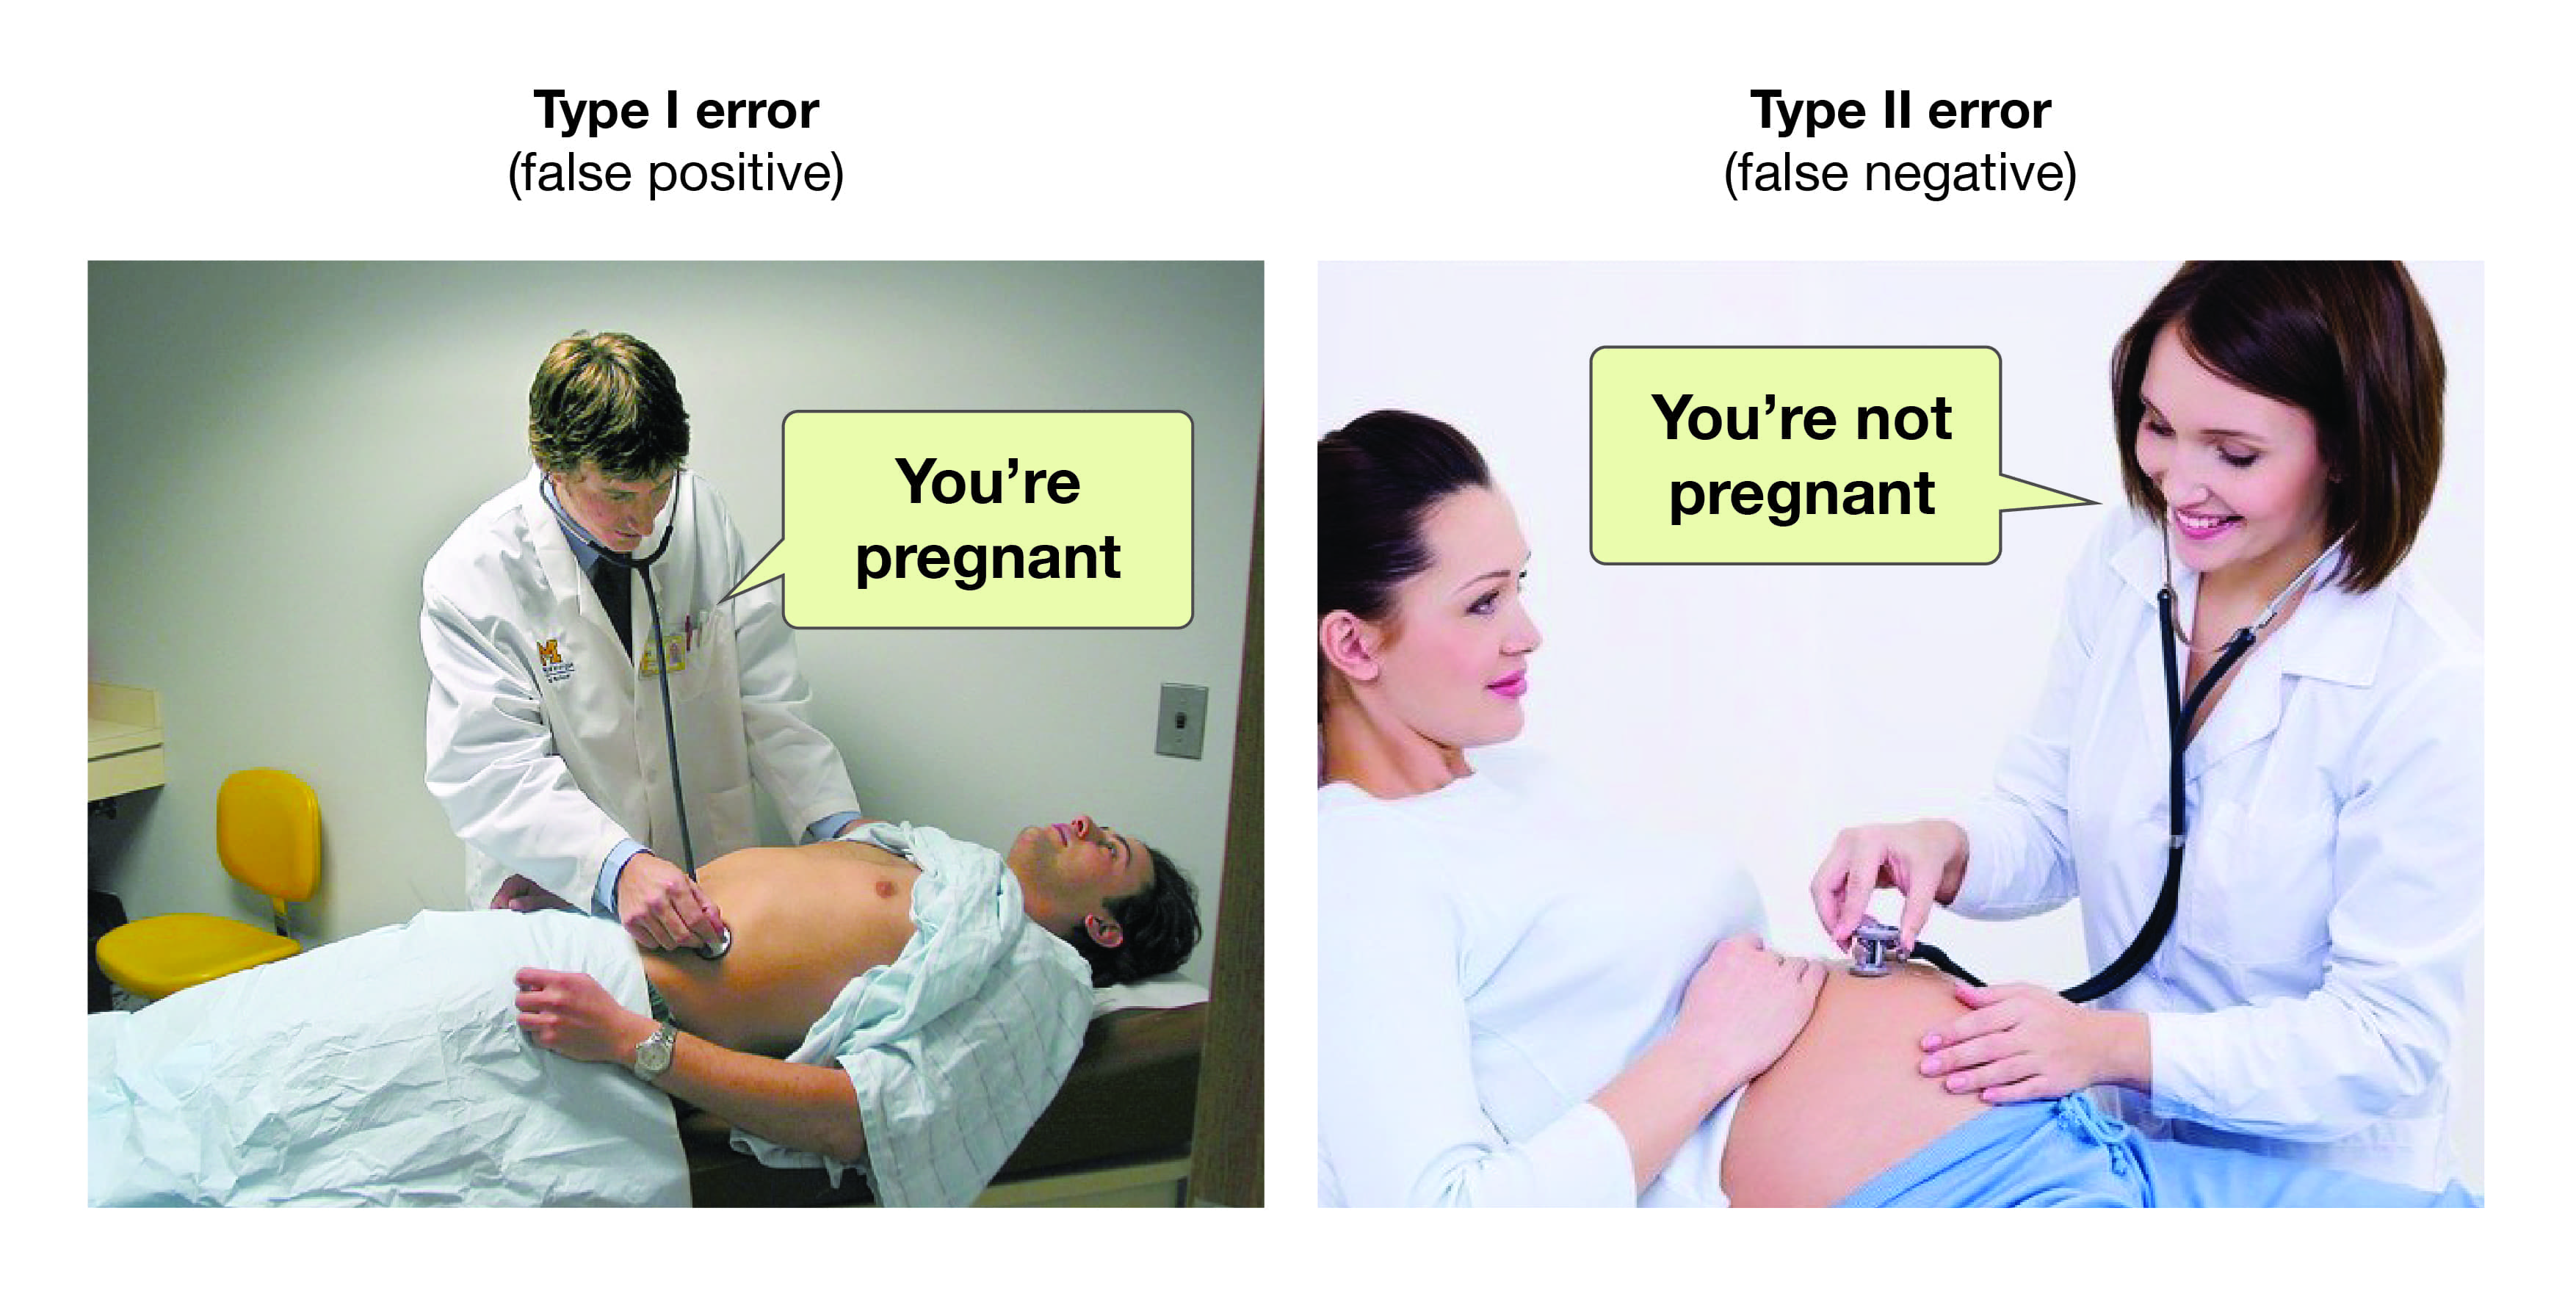
\includegraphics[width=0.9\linewidth]{images/results/bin_type_errors.jpeg}
    \caption{The gravity of an error depends on the contest in which it happens. False Negatives and False Positives can have different gravity.}
    \label{fig:bin-errors}
\end{figure}

Starting from the primitive metrics, it is possible to compute more complex evaluation metrics, such as Recall, Specificity, and Precision.\\
\textbf{Recall}, also called True Positive Rate or Sensitivity, represents how many relevant items are selected.\\
\textbf{Specificity}, also called False Positive Rate, represents how many negative elements are truly negative.\\
\textbf{Precision} represents how many selected items are relevant.\\
These metrics are calculated as follows:

\begin{equation}
    \begin{aligned}
    Recall &= \frac{TP}{TP + FN}\\[10pt]
    Specificity &= \frac{TN}{TN + FP}\\[10pt]
    Precision &= \frac{TP}{TP + FP}\\[10pt]
    \end{aligned}
\end{equation}

where $TP, TN, FP, FN$ are respectively True Positives, True Negatives, False Positives, and False Negatives.

\noindent Recall, Specificity, and Precision may not be enough to evaluate a classifier, so they are often combined into other metrics, such as F\textsubscript{1}-Score, IoU, and D\textsubscript{prs}.\\
\textbf{F\textsubscript{1}-Score}, also called F-Measure, Sørensen-Dice coefficient, or Dice similarity coefficient, is a measure of a test's accuracy.
The F\textsubscript{1} in its name means that the $\beta$ value of the generic F-Score is set to 1.
The $F_1$ score is the harmonic mean of precision and recall.
The more generic $F_\beta$ score applies additional weights, valuing one of precision or recall more than the other.\\
\textbf{Intersection Over Union (IoU)}, also named Jaccard index, measures similarity between finite sample sets, and is defined as the size of the intersection divided by the size of the union of the sample sets. The sample sets are represented by the ground truth and the prediction given by a skin detector.\\
\textbf{D\textsubscript{prs}}~\cite{intawong2013new} is a metric that focuses on segmentation algorithms. The already mentioned metrics are expressed as a compromise between two of the three aspects that are important for a quality assessment: Precision, Recall, and Specificity~\cite{intawong2013new}.
D\textsubscript{prs} takes into account all of the three aspects.
It measures the Euclidean distance between the segmentation, represented by the point $(PR, RE, SP)$, and the ground truth, the ideal point $(1, 1, 1)$, hence lower values are better in this case.\\
These metrics are calculated as follows:

\begin{equation}
    \begin{aligned}
    F_1&=\frac{2 T P}{2 T P+F P+F N}\\[10pt]
    IoU&=\frac{T P}{T P+F P+F N}\\[10pt]
    D_{p r s}&=\sqrt{(1-P R)^{2}+(1-R E)^{2}+(1-S P)^{2}}\\[10pt]
    \end{aligned}
\end{equation}

where $PR, RE, SP$ are Precision, Recall, and Specificity, respectively.

\noindent It is possible to note that F\textsubscript{1}-Score and IoU have a similar formula: the only difference is that  F\textsubscript{1} weights the True Positives higher.
When taking the average score of each metric over a set of inferences, IoU tends to penalize single instances of bad classification more than the F\textsubscript{1} score~\footnote{A detailed explanation can be found at \url{https://stats.stackexchange.com/a/276144}}.
Suppose for example that the vast majority of the inferences are moderately better with classifier A than B, but some of them are significantly worse using classifier A. It may be the case then that the F\textsubscript{1} metric favors classifier A while the IoU metric favors classifier B.
For a better interpretation of the average scores between multiple instances, the difference \textbf{F\textsubscript{1}-IoU} is taken into account.
The higher the difference, the more is the bad inferences in the set, while a lower difference means that the prediction set is more balanced.
All the described metrics range from 0 to 1, except for primitives, which are whole numbers, and D\textsubscript{prs}, which ranges from 0 to $\sqrt{3}$.

\noindent It is also important to note that F\textsubscript{1} and IoU do not take into account the True Negatives. In the case of skin detection the performances are generally measured on the skin class, hence this limitation is negligible. However, if True Negatives are important for an evaluation, more balanced metrics should be taken into account, such as the Matthews correlation coefficient (MCC)~\cite{chicco2020advantages}.


%%%%%%%%%%%%%%%%%%%%%%%%%%%%%%%%%%%%%%%%%%%%%%%%%%%%%%%%%%%%%%%%%%%%%%%%
\section{Experimental setup}
%%%%%%%%%%%%%%%%%%%%%%%%%%%%%%%%%%%%%%%%%%%%%%%%%%%%%%%%%%%%%%%%%%%%%%%%

% VALIDATION
Before the evaluation process on the chosen datasets, the selected methods have been validated on the datasets splits used in their original papers.
In this way, it has been possible to check their proper functioning.
The statistical method~\cite{acharjee2018skin} has not been validated because it does not refer to a paper and evaluations are not reported.
The thresholding method~\cite{brancati2017human} uses a metrics averaging of this type: the Recall, Precision, and Specificity measures are calculated as average scores over the set of instances, then the obtained scores are used to calculate F\textsubscript{1}-Score and D\textsubscript{prs}.
The U-Net approach~\cite{tarasiewicz2020skinny}, instead, calculates the F\textsubscript{1}-Score directly as the average score over all the set of instances.
The validation results are shown in \autoref{tab:methods-val-dyc}
and \autoref{tab:methods-val-skinny}.

\begin{table}[h]
    \centering
    \resizebox{\columnwidth}{!}{
        \begin{tabular}{l@{\hskip 12mm}ccc@{\hskip 8mm}ccc}
        \toprule
        & \multicolumn{3}{c}{F\textsubscript{1}-Score} & \multicolumn{3}{c}{D\textsubscript{prs}}\\
        & HGR\textsuperscript{1} & ECU & Pratheepan & HGR\textsuperscript{1} & ECU & Pratheepan\\
        \midrule
        Original & \monosp{0.8252} & \monosp{0.6550} & \monosp{0.6592} & \monosp{0.2667} & \monosp{0.5043} & \monosp{0.5149}\\
        Implementation & \monosp{0.8257} & \monosp{0.6586} & \monosp{0,6630} & \monosp{0.2660} & \monosp{0.5006} & \monosp{0.5096}\\
        \midrule
        Change & \monosp{0.0005} & \monosp{0.0036} & \monosp{0.0038} & \monosp{0.0007} & \monosp{0.0037} & \monosp{0.0053}\\
        \bottomrule
        \end{tabular}}
    \caption{Brancati \textit{et al.} 2017~\cite{brancati2017human} validation data.\\
    Each dataset was used in its entirety to perform the testing.\\
    \textsuperscript{1}HGR consists of: HGR1, HGR2A-downscaled, HGR2B-downscaled.}
    \label{tab:methods-val-dyc}
\end{table}

\begin{table}[h]
    \centering
    %\resizebox{\columnwidth}{!}{
        \begin{tabular}{l@{\hskip 12mm}cc}
        \toprule
        & \multicolumn{2}{c}{F\textsubscript{1}-Score}\\
        & HGR\textsuperscript{1} & ECU\textsuperscript{2}\\
        \midrule
        Original & \monosp{0.9494} & \monosp{0.9230}\\
        Implementation & \monosp{0.9308}  & \monosp{0.9133}\\
        \midrule
        Change & \monosp{0.0186} & \monosp{0.0097}\\
        \bottomrule
        \end{tabular}%}
    \caption{Tarasiewicz \textit{et al.} 2020~\cite{tarasiewicz2020skinny} validation data.\\
    \textsuperscript{1}HGR consists of: HGR1, HGR2A-downscaled, HGR2B-downscaled.\\
    \textsuperscript{2}ECU was split accordingly to the original work of the method.\\
    The model was trained on the ECU splits; HGR has not been used for training.\\
    The testing was performed on the test set of ECU and the entirety of HGR.}
    \label{tab:methods-val-skinny}
\end{table}


% DATASETS
After the validation phase, the setup of the experiments begins with the definition of the employed datasets:
\begin{itemize}
    \item ECU: 3998 images.
    \item HGR: 1558 images from HGR1, HGR2A-downscaled, HGR2B-downscaled sub-datasets.
    \item Schmugge: 840 images.
    The pictures have been processed by reading the \path{.config.SkinImManager} file provided by the dataset.
    Five pictures have been ignored because of faulty ground truths: \path{aa50.gt.d3}, \path{dd71.gt.d3}, \path{hh54.gt.d3}, and \path{aa69.gt.d3} that has a duplicated entry in the file.
    The rule used to manage the ternary ground truths has been considering whatever is not the background as skin.
\end{itemize}

\noindent Skin tones sub-datasets are defined by taking advantage of the additional labels in the Schmugge dataset.
The resulting sub-datasets represent light, medium, and dark skin tones and consist of 409, 101, and 27 pictures, respectively.
Not all Schmugge dataset is used for skin tones, because the database contains whole images of non-skin pixels, as described in \autoref{sec:chosen-datasets}.

None of the datasets provide native training and testing splits.
The train and validation sets have been merged in methods that do not use the validation set.
For ECU, the splits used are the ones mentioned in Tarasiewicz \textit{et al.} 2020~\cite{tarasiewicz2020skinny}.
HGR, Schmugge, and skin tone splits are randomly defined by keeping the following proportions: 70\% train, 15\% validation, and 15\% test.
Since the proportions would reduce the dark sub-dataset to only 19 training images, the data has been augmented in this case, only for the training split.
The purpose is to get at least 100 images for the evaluations, but also to generate images that look natural; 104 was the final size of the training set.
The following augmentation operations provided by the Albumentations library~\cite{buslaev2020albumentations} are performed in the following order:
\begin{itemize}
\itemsep0em
    \item \path{HorizontalFlip(p=1)} on original images.
    \item \path{Rotate(limit = 15, p=0.8)} on the original images plus the ones obtained by the horizontal flipping.
    \item \path{RandomCrop(H*0.8, W*0.8, p=0.8)} on the original images plus the ones obtained by the horizontal flipping plus the ones obtained by the rotation.
\end{itemize}
where \path{H} and \path{W} are the height and width of the processed image, respectively, and \path{p} and \path{limit} are the probability that the transformation happens, and the rotation limits in degrees (the angle is between \path{-limit} and \path{+limit}), respectively.


% METHODS
Once the datasets have been defined, the settings of the methods can be adjusted.
The thresholding~\cite{brancati2017human} and statistical~\cite{acharjee2018skin} approaches have been left to their default implementations settings described in \autoref{sec:impl-thresh} and \autoref{sec:impl-bayes}, respectively.
The U-Net approach~\cite{tarasiewicz2020skinny} uses only the complete model named \q{Skinny} with the following settings:
\begin{itemize}
    \item Maximum number of epochs = 200
    \item Batch size = 3
    \item Initial learning rate = $10^{-4}$
    \item Minimum learning rate = $10^{-6}$
    \item Reduce learning rate on plateau patience = 5
    \item Early stopping patience = 10 for HGR, ECU, and Schmugge models.\\
    Early stopping patience = 50 for light, medium, dark models (by having only 4 validation images in the dark sub-dataset, the model has a harder time taking the right path).
    \item Adam~\cite{kingma2014adam} optimizer with $\beta_1 = 0.9$ and $\beta_2 = 0.999$
    \item The loss function is the average of Binary Cross-Entropy and the Dice coefficient.
    \item The original preprocessing: the images with over $(512 \times 512)$ pixels are downscaled preserving the aspect ratio so that the number of pixels does not exceed $(512 \times 512)$. Moreover, Skinny applies a padding operation after the possible downscale to make the width and height of images multiple of 32, as seen in \autoref{fig:skinny-padding}.
    \item The models have been trained by monitoring the F\textsubscript{1} over the validation set and saving on new max values.
\end{itemize}


% EVALUATION
\noindent The last phase of the setup is defining the evaluation process.
Some methods did not provide a binary prediction, but a prediction with grayscale values. All the predictions have been binarized by rounding each pixel value to either be white or black.
%By having a binarized ground truth and a binarized prediction, metrics measurement is possible.
Initially, the metrics are measured for all the instances, then the average and population standard deviation for each metric are computed.

% cross, base, performance
Two different settings of dataset evaluation are performed: single and cross evaluation.
The first measures how well a method performs with respect to the same dataset, the second measures how well a method generalizes with respect to other datasets.\\
In the \textbf{single evaluation} of a method over a dataset, the method is eventually trained on the training set, in the case of a trainable method, and then predictions are performed on the test set.\\
In the \textbf{cross evaluation}, only the trainable approaches are analyzed.
The models are the same of the single evaluation: each model is trained on the training set of a dataset.
The evaluation of a method is performed over the whole dataset by the models that have not been trained on the concerning dataset.

\begin{figure}[h]
     \centering
     \begin{subfigure}[b]{0.23\textwidth}
         \centering
         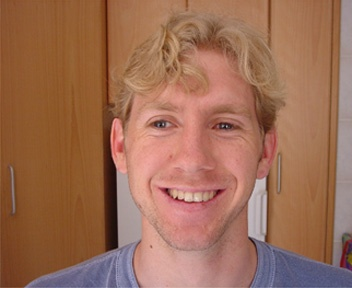
\includegraphics[width=\textwidth]{images/results/unet_padding_im00060_x.jpg}
         \caption{}
     \end{subfigure}
     \hfill
     \begin{subfigure}[b]{0.23\textwidth}
         \centering
         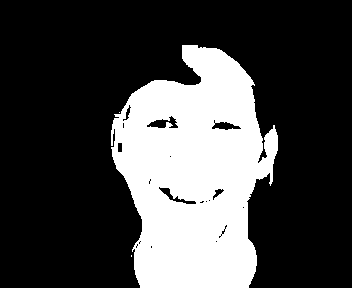
\includegraphics[width=\textwidth]{images/results/unet_padding_im00060_y.png}
         \caption{}
     \end{subfigure}
    \hfill
     \begin{subfigure}[b]{0.23\textwidth}
         \centering
         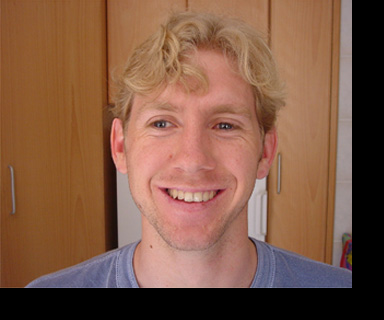
\includegraphics[width=\textwidth]{images/results/unet_padding_1311x.png}
         \caption{}
     \end{subfigure}
    \hfill
     \hfill
     \begin{subfigure}[b]{0.23\textwidth}
         \centering
         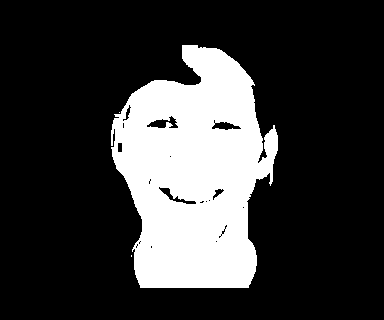
\includegraphics[width=\textwidth]{images/results/unet_padding_1311y.png}
         \caption{}
     \end{subfigure}
        \caption{Skinny~\cite{tarasiewicz2020skinny} applies padding to make the width and height of an image a multiple of 32. If the dimensions of the image are already a multiple of 32, a padding of 32 is still applied.
        (a) original image; (b) ground truth; (c) preprocessed original image; (d) preprocessed ground truth}
        \label{fig:skinny-padding}
\end{figure}


\FloatBarrier
%%%%%%%%%%%%%%%%%%%%%%%%%%%%%%%%%%%%%%%%%%%%%%%%%%%%%%%%%%%%%%%%%%%%%%%%
\section{Performance on single databases}
%%%%%%%%%%%%%%%%%%%%%%%%%%%%%%%%%%%%%%%%%%%%%%%%%%%%%%%%%%%%%%%%%%%%%%%%

In the single evaluation of the datasets, \autoref{tab:base-normal}, the deep-learning approach beats its competitors in all the measurements, while the statistical approach comes always second.
The Schmugge dataset describes a higher difficulty of classification that can be attributed to the variety of the lighting conditions, subjects, and environments present in its pictures.
The variety of the database can also be described by the high standard deviation measurements obtained.
Furthermore, by considering the ambiguous regions as skin pixels, the performance of the classifier may be affected.
The high D\textsubscript{prs} scores obtained by the statistical and thresholding methods may indicate the presence of many True Negatives, as the metric is the only one between the chosen metrics that incorporates them.
HGR seems to be the easier dataset to classify, which can be due to the relatively low diversity of subjects and backgrounds. In fact, learning approaches tend to have very high measurements.
Tarasiewicz \textit{et al.} 2020~\cite{tarasiewicz2020skinny} seems to perform very well on this dataset, achieving very low standard deviation scores.
In the ECU dataset, the results of the histogram and thresholding approaches are relatively close, while the CNN outperforms them by far.

Some interesting instances can be seen in \autoref{fig:base-normal-samples}.
The first row shows the problem that having a background with similar colors to the skin represents in the color-based methods.
The statistical method seems to act relatively better in this scenario compared to Brancati \textit{et al.} 2017~\cite{brancati2017human}, as seen in the second row.
In the third row, the statistical approach classify some background and hair pixels as skin, while the rule-based method has many False Negatives, but the head remain still recognizable.
The fourth row represent a very hard image to classify.
Interestingly, the U-Net describes a very bad classifications, with a tremendous number of False Positives.
The thresholding approach is the most restrictive on False Positives in this instance.
The next-to-last image has an inconvenient background with skin-like colors and only Tarasiewicz \textit{et al.} 2020~\cite{tarasiewicz2020skinny} tend to have a good classification.
The statistical method manages to classify the skin pixels well, but has a really high number of False Positives.
The last image is a landscape image without skin pixels and once again the color-based approaches describe many False Positives, with the machine learning one having lots of them.

\begin{table}[ht]
    \centering
    \resizebox{\columnwidth}{!}{
    \begin{tabular}{clccc}
    \toprule
    & Method\textbackslash Database & ECU & HGR & Schmugge \\
    \midrule
    %
    %
    \multirow{3}{*}{{$F_1 \uparrow$}}
        & Tarasiewicz \textit{et al.}~\cite{tarasiewicz2020skinny}
        & $\pmb{0.9133 \pm 0.08}$ & $\pmb{0.9848 \pm 0.02}$ & $\pmb{0.6121 \pm 0.45}$ \\
        %
        & Acharjee~\cite{acharjee2018skin}
        & $\underline{0.6980 \pm 0.22}$ & $\underline{0.9000 \pm 0.15}$ & $\underline{0.5098 \pm 0.39}$ \\
        %
        & Brancati \textit{et al.}~\cite{brancati2017human}
        & $0.6356 \pm 0.24$ & $0.7362 \pm 0.27$ & $0.4280 \pm 0.34$ \\[5pt]
        %
        %
    \multirow{3}{*}{{$IoU \uparrow$}}
        & Tarasiewicz \textit{et al.}~\cite{tarasiewicz2020skinny}
        & $\pmb{0.8489 \pm 0.12}$ & $\pmb{0.9705 \pm 0.03}$ & $\pmb{0.5850 \pm 0.44}$ \\
        %
        & Acharjee~\cite{acharjee2018skin}
        & $\underline{0.5751 \pm 0.23}$ & $\underline{0.8434 \pm 0.19}$ & $\underline{0.4303 \pm 0.34}$ \\
        %
        & Brancati \textit{et al.}~\cite{brancati2017human}
        & $0.5088 \pm 0.25$ & $0.6467 \pm 0.30$ & $0.3323 \pm 0.28$ \\[5pt]
        %
        %
    \multirow{3}{*}{{$D_{prs} \downarrow$}}
        & Tarasiewicz \textit{et al.}~\cite{tarasiewicz2020skinny}
        & $\pmb{0.1333 \pm 0.12}$ & $\pmb{0.0251 \pm 0.03}$ & $\pmb{0.5520 \pm 0.64}$ \\
        %
        & Acharjee~\cite{acharjee2018skin}
        & $\underline{0.4226 \pm 0.27}$ & $\underline{0.1524 \pm 0.19}$ & $\underline{0.7120 \pm 0.54}$ \\
        %
        & Brancati \textit{et al.}~\cite{brancati2017human}
        & $0.5340 \pm 0.32$ & $0.3936 \pm 0.36$ & $0.8148 \pm 0.48$\\
        %
        %
    \bottomrule
    \end{tabular}}
    \caption{Single evaluation on datasets.\\
        For each dataset: methods are eventually trained on the training set, in the case of trainable methods, and then predictions are performed on the test set.\\
        For example, with ECU as the dataset, it means that a method is trained using the training set of ECU, if the method is trainable, and then tested on the test set of ECU.}
    \label{tab:base-normal}
\end{table}

\begin{figure}[h]
     \centering
     % ROW 1
     \begin{subfigure}[b]{0.18\textwidth}
         \centering
         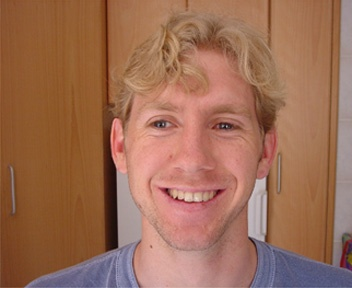
\includegraphics[width=\textwidth]{images/results/base/im00060_x.jpg}
     \end{subfigure}
     \hfill
     \begin{subfigure}[b]{0.18\textwidth}
         \centering
         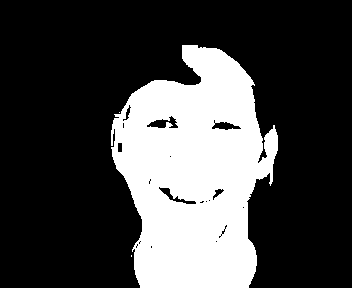
\includegraphics[width=\textwidth]{images/results/base/im00060_y.png}
     \end{subfigure}
    \hfill
     \begin{subfigure}[b]{0.18\textwidth}
         \centering
         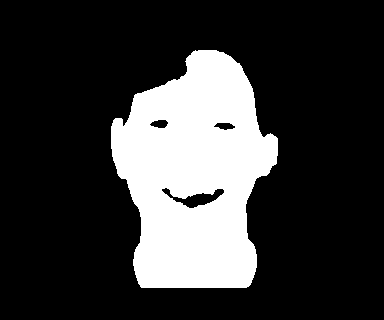
\includegraphics[width=\textwidth]{images/results/base/im00060_skinny_1311.png}
     \end{subfigure}
    \hfill
     \begin{subfigure}[b]{0.18\textwidth}
         \centering
         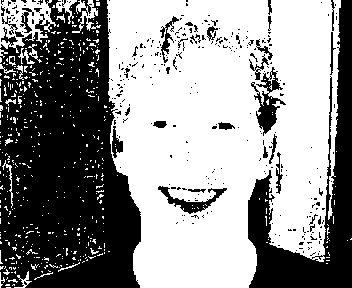
\includegraphics[width=\textwidth]{images/results/base/im00060_bayes_base_ecu.png}
     \end{subfigure}
    \hfill
     \begin{subfigure}[b]{0.18\textwidth}
         \centering
         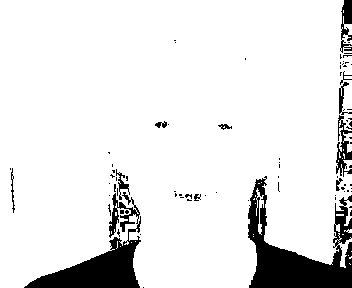
\includegraphics[width=\textwidth]{images/results/base/im00060_dyc_base_ecu.png}
     \end{subfigure}
     % ROW 2
     \begin{subfigure}[b]{0.18\textwidth}
         \centering
         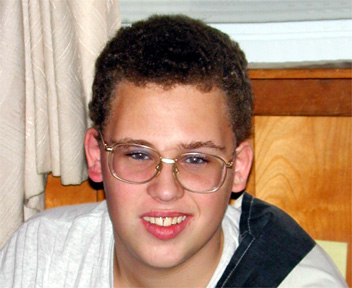
\includegraphics[width=\textwidth]{images/results/base/im00077_x.jpg}
     \end{subfigure}
     \hfill
     \begin{subfigure}[b]{0.18\textwidth}
         \centering
         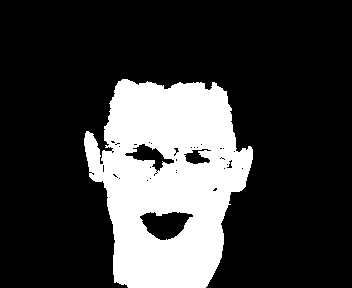
\includegraphics[width=\textwidth]{images/results/base/im00077_y.png}
     \end{subfigure}
    \hfill
     \begin{subfigure}[b]{0.18\textwidth}
         \centering
         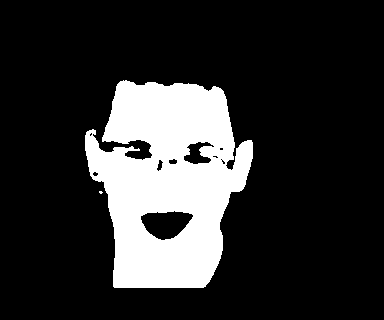
\includegraphics[width=\textwidth]{images/results/base/im00077_skinny_1272.png}
     \end{subfigure}
    \hfill
     \begin{subfigure}[b]{0.18\textwidth}
         \centering
         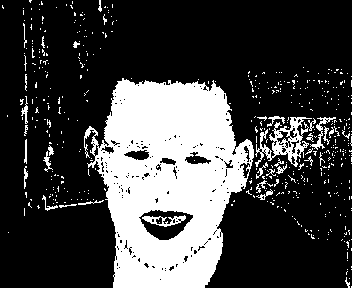
\includegraphics[width=\textwidth]{images/results/base/im00077_bayes.png}
     \end{subfigure}
     \hfill
     \begin{subfigure}[b]{0.18\textwidth}
         \centering
         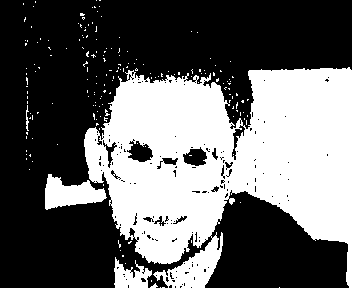
\includegraphics[width=\textwidth]{images/results/base/im00077_dyc.png}
     \end{subfigure}
     % ROW 3
     \begin{subfigure}[b]{0.18\textwidth}
         \centering
         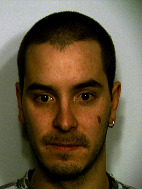
\includegraphics[width=\textwidth]{images/results/base/hh78.color.d3_x.png}
     \end{subfigure}
     \hfill
     \begin{subfigure}[b]{0.18\textwidth}
         \centering
         
\includegraphics[width=\textwidth]{images/results/base/hh78.color.d3_y.png}
     \end{subfigure}
    \hfill
     \begin{subfigure}[b]{0.18\textwidth}
         \centering
         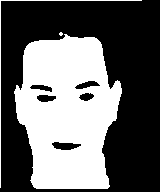
\includegraphics[width=\textwidth]{images/results/base/hh78.color.d3_skinny_5.png}
     \end{subfigure}
    \hfill
     \begin{subfigure}[b]{0.18\textwidth}
         \centering
         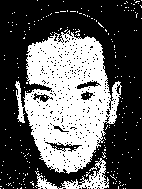
\includegraphics[width=\textwidth]{images/results/base/hh78.color.d3_bayes.png}
     \end{subfigure}
    \hfill
     \begin{subfigure}[b]{0.18\textwidth}
         \centering
         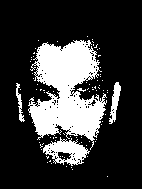
\includegraphics[width=\textwidth]{images/results/base/hh78.color.d3_dyc.png}
     \end{subfigure}
     % ROW 4
     \begin{subfigure}[b]{0.18\textwidth}
         \centering
         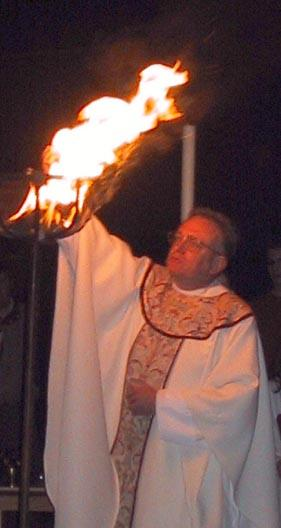
\includegraphics[width=\textwidth]{images/results/base/lighting_fire_x.png}
     \end{subfigure}
     \hfill
     \begin{subfigure}[b]{0.18\textwidth}
         \centering
         
\includegraphics[width=\textwidth]{images/results/base/lighting_fire_y.png}
     \end{subfigure}
    \hfill
     \begin{subfigure}[b]{0.18\textwidth}
         \centering
         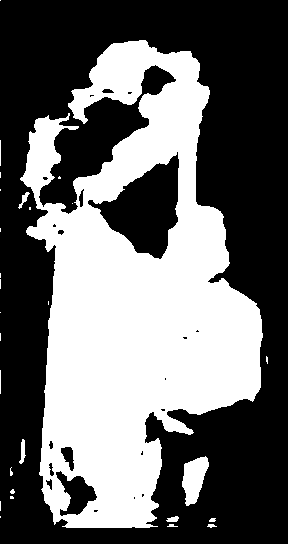
\includegraphics[width=\textwidth]{images/results/base/lighting_fire_skinny_115.png}
     \end{subfigure}
    \hfill
     \begin{subfigure}[b]{0.18\textwidth}
         \centering
         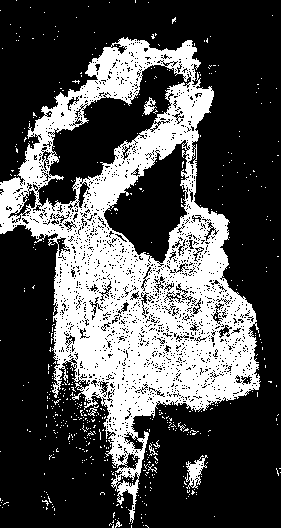
\includegraphics[width=\textwidth]{images/results/base/lighting_fire_bayes.png}
     \end{subfigure}
    \hfill
     \begin{subfigure}[b]{0.18\textwidth}
         \centering
         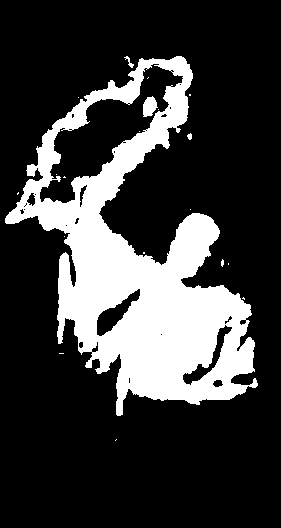
\includegraphics[width=\textwidth]{images/results/base/lighting_fire_dyc.png}
     \end{subfigure}
     % ROW 5
     \begin{subfigure}[b]{0.18\textwidth}
         \centering
         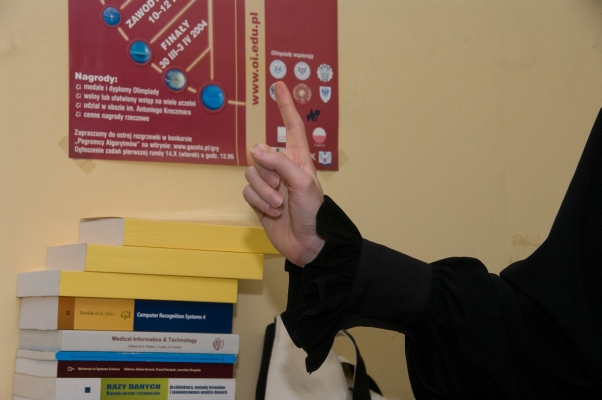
\includegraphics[width=\textwidth]{images/results/base/1_A_hgr2A2_id01_1_x.jpg}
     \end{subfigure}
     \hfill
     \begin{subfigure}[b]{0.18\textwidth}
         \centering
         
\includegraphics[width=\textwidth]{images/results/base/1_A_hgr2A2_id01_1_y.png}
     \end{subfigure}
    \hfill
     \begin{subfigure}[b]{0.18\textwidth}
         \centering
         
\includegraphics[width=\textwidth]{images/results/base/1_A_hgr2A2_id01_1_skinny_8.png}
     \end{subfigure}
    \hfill
     \begin{subfigure}[b]{0.18\textwidth}
         \centering
         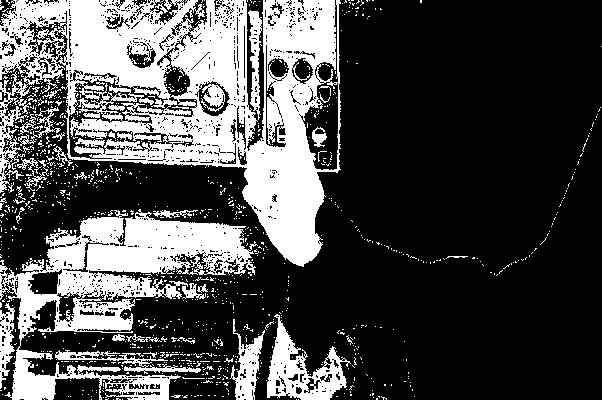
\includegraphics[width=\textwidth]{images/results/base/1_A_hgr2A2_id01_1_bayes.png}
     \end{subfigure}
    \hfill
     \begin{subfigure}[b]{0.18\textwidth}
         \centering
         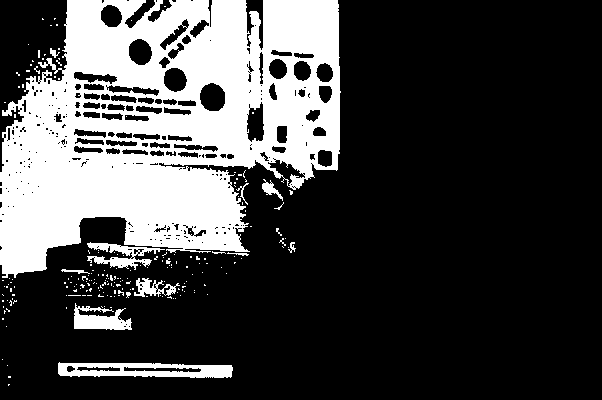
\includegraphics[width=\textwidth]{images/results/base/1_A_hgr2A2_id01_1_dyc.png}
     \end{subfigure}
     % ROW 6
     \begin{subfigure}[b]{0.18\textwidth}
         \centering
         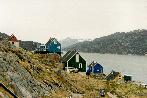
\includegraphics[width=\textwidth]{images/results/base/greenland.205.color.d3_x.png}
         \caption{}
     \end{subfigure}
     \hfill
     \begin{subfigure}[b]{0.18\textwidth}
         \centering
         
\includegraphics[width=\textwidth]{images/results/base/greenland.205.color.d3_y.png}
         \caption{}
     \end{subfigure}
    \hfill
     \begin{subfigure}[b]{0.18\textwidth}
         \centering
         
\includegraphics[width=\textwidth]{images/results/base/greenland.205.color.d3_skinny.png}
         \caption{}
     \end{subfigure}
    \hfill
     \begin{subfigure}[b]{0.18\textwidth}
         \centering
         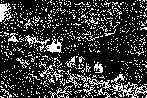
\includegraphics[width=\textwidth]{images/results/base/greenland.205.color.d3_bayes.png}
         \caption{}
     \end{subfigure}
     \hfill
     \begin{subfigure}[b]{0.18\textwidth}
         \centering
         
\includegraphics[width=\textwidth]{images/results/base/greenland.205.color.d3_dyc.png}
         \caption{}
     \end{subfigure}
        \caption{Skin detection results in datasets single evaluation: (a) the input image; (b) the ground truth; (c) Tarasiewicz \textit{et al.} 2020~\cite{tarasiewicz2020skinny}; (d) Acharjee~\cite{acharjee2018skin}; (e) Brancati \textit{et al.} 2017~\cite{brancati2017human}.\\
        In all the following results, Tarasiewicz \textit{et al.} 2020~\cite{tarasiewicz2020skinny} predictions have different dimensions than other images due to the network preprocessing.}
        \label{fig:base-normal-samples}
\end{figure}


\FloatBarrier
%%%%%%%%%%%%%%%%%%%%%%%%%%%%%%%%%%%%%%%%%%%%%%%%%%%%%%%%%%%%%%%%%%%%%%%%
\section{Performance across databases}
%%%%%%%%%%%%%%%%%%%%%%%%%%%%%%%%%%%%%%%%%%%%%%%%%%%%%%%%%%%%%%%%%%%%%%%%

In the cross evaluation of the datasets (present at \autoref{tab:cross-normal}), the deep learning approach still dominates, but there are some interesting exceptions.
In fact, using HGR as the training set and predicting over Schmugge, Acharjee 2018~\cite{acharjee2018skin} outperforms Tarasiewicz \textit{et al.} 2020~\cite{tarasiewicz2020skinny}, especially in the F\textsubscript{1} score.
This means that, while the statistical method generally performs better than Tarasiewicz \textit{et al.} 2020~\cite{tarasiewicz2020skinny}, it also includes a lot of False Positives, as the F\textsubscript{1}-IoU and the D\textsubscript{prs} metrics indicate.
The latter is particularly bad in both cases, evidencing a big distance between the ideal ground truths and the predictions.
In the case where ECU is used to train and Schmugge to predict, and in the opposite case, Tarasiewicz \textit{et al.} 2020~\cite{tarasiewicz2020skinny} beats the statistical method discretely.
In the latter case, the U-Net describes a slightly worse F\textsubscript{1}-IoU, suggesting the presence of False Positives and False Negatives.
Tarasiewicz \textit{et al.} 2020~\cite{tarasiewicz2020skinny} outperforms the other machine learning approach by far in the remaining cases.
The U-Net exceeds an F\textsubscript{1} score of 80 in the case of Schmugge as the training set and HGR as the prediction set despite the size of the training set, which is not huge.

\begin{table}[ht]
    \centering
    \resizebox{\columnwidth}{!}{
        \begin{tabular}{clcccccc}
        \toprule
        \multicolumn{1}{c}{} & \multicolumn{1}{c}{Training} 
        & \multicolumn{2}{c}{ECU} & \multicolumn{2}{c}{HGR} & \multicolumn{2}{c}{SCHMUGGE} \\\multicolumn{1}{c}{} & \multicolumn{1}{c}{Testing}  & \multicolumn{1}{c}{HGR}  & \multicolumn{1}{c}{SCHMUGGE}  & \multicolumn{1}{c}{ECU}  & \multicolumn{1}{c}{SCHMUGGE}  & \multicolumn{1}{c}{ECU}  & \multicolumn{1}{c}{HGR} \\
        \midrule\multirow{2}{*}{{$F_1$ $\uparrow$}}& Taras. \textit{et al.}~\cite{tarasiewicz2020skinny}\rule{0pt}{14pt} & \monosp{\monobold{0.9308 \pm 0.11}} & \monosp{\monobold{0.4625 \pm 0.41}} & \monosp{\monobold{0.7252 \pm 0.20}} & \monosp{0.2918 \pm 0.31} & \monosp{\monobold{0.6133 \pm 0.21}} & \monosp{\monobold{0.8106 \pm 0.19}}\\& Acharjee~\cite{acharjee2018skin} & \monosp{0.5577 \pm 0.29} & \monosp{0.3319 \pm 0.28} & \monosp{0.4279 \pm 0.19} & \monosp{\monobold{0.4000 \pm 0.32}} & \monosp{0.4638 \pm 0.23} & \monosp{0.5060 \pm 0.25}\\\multirow{2}{*}{{$IoU$ $\uparrow$}}& Taras. \textit{et al.}~\cite{tarasiewicz2020skinny}\rule{0pt}{14pt} & \monosp{\monobold{0.8851 \pm 0.15}} & \monosp{\monobold{0.3986 \pm 0.37}} & \monosp{\monobold{0.6038 \pm 0.22}} & \monosp{0.2168 \pm 0.25} & \monosp{\monobold{0.4754 \pm 0.22}} & \monosp{\monobold{0.7191 \pm 0.23}}\\& Acharjee~\cite{acharjee2018skin} & \monosp{0.4393 \pm 0.27} & \monosp{0.2346 \pm 0.21} & \monosp{0.2929 \pm 0.17} & \monosp{\monobold{0.2981 \pm 0.24}} & \monosp{0.3318 \pm 0.20} & \monosp{0.3752 \pm 0.22}\\\multirow{2}{*}{{$D_{prs}$ $\downarrow$}}& Taras. \textit{et al.}~\cite{tarasiewicz2020skinny}\rule{0pt}{14pt} & \monosp{\monobold{0.1098 \pm 0.15}} & \monosp{\monobold{0.7570 \pm 0.56}} & \monosp{\monobold{0.3913 \pm 0.26}} & \monosp{\monobold{0.9695 \pm 0.44}} & \monosp{\monobold{0.5537 \pm 0.27}} & \monosp{\monobold{0.2846 \pm 0.27}}\\& Acharjee~\cite{acharjee2018skin} & \monosp{0.5701 \pm 0.29} & \monosp{1.0477 \pm 0.35} & \monosp{0.8830 \pm 0.23} & \monosp{1.0219 \pm 0.42} & \monosp{0.7542 \pm 0.30} & \monosp{0.6523 \pm 0.27}\\\multirow{2}{*}{{$F_1 - IoU$ $\downarrow$}}& Taras. \textit{et al.}~\cite{tarasiewicz2020skinny}\rule{0pt}{14pt} & \monosp{\monobold{0.0457}} & \monosp{\monobold{0.0639}} & \monosp{\monobold{0.1214}} & \monosp{\monobold{0.0750}} & \monosp{0.1379} & \monosp{\monobold{0.0915}}\\& Acharjee~\cite{acharjee2018skin} & \monosp{0.1184} & \monosp{0.0973} & \monosp{0.1350} & \monosp{0.1019} & \monosp{\monobold{0.1320}} & \monosp{0.1308}\\
        \bottomrule
        \end{tabular}}
    \caption{Cross evaluation on datasets.\\
        For each dataset: methods are trained on the training set and then predictions are performed on all the images of every other datasets.\\
        For example, with ECU as the training dataset and HGR as the testing dataset, it means that a method is trained using the training set of ECU, and then tested on all the HGR dataset.}
    \label{tab:cross-normal}
\end{table}

Some interesting instances are shown in \autoref{fig:cross-normal-samples}.
The expression \q{HGR on ECU} describes the situation in which the evaluation is performed by using HGR as the training set and ECU as the test set. In cross evaluations, this type of expression is going to be used a lot to avoid text redundancy.
The first row (HGR on ECU) shows a really poor classification by the statistical approach.
In the second row (ECU on Schmugge) it can be noticed how Acharjee 2018~\cite{acharjee2018skin} tends to exaggerate at classifying skin pixels in some cases, confirming the above intuitions on the statistical method having a lot of False Positives.
The third row (ECU on Schmugge) describes a tragic classification by Tarasiewicz \textit{et al.} 2020~\cite{tarasiewicz2020skinny}, that might be caused by the presence of tricky lighting conditions and shadows on the skin regions.
The statistical approach performs badly too, but still has a lot better classification.
In this case, the ground truth shows how incorporating the ambiguous regions provided by the Schmugge database makes the skin regions quite pixels-hungry on the border with non-skin regions.
The fourth image (Schmugge on ECU) represents a bad classification in both approaches, where there is especially an outstanding number of False Positives.
The next-to-last image (HGR on Schmugge) is part of the datasets combination in which Acharjee 2018~\cite{acharjee2018skin} outperforms the deep learning one.
The statistical method reports a lot of False Positives, but also a lot of True Positives, which Tarasiewicz \textit{et al.} 2020~\cite{tarasiewicz2020skinny} struggles to identify.
The last picture (HGR on Schmugge) is also part of the same datasets combination and describes a similar situation: the U-Net fails at labeling several skin pixels, especially on very lit regions, while the statistical method overdoes it.
This image represents the high complexity and diversity of the Schmugge content.

\begin{figure}[h]
     \centering
     
     \resizebox{0.8\textwidth}{0.17\textheight}{
     % ROW 1
     \begin{subfigure}[b]{0.23\textwidth}
         \centering
         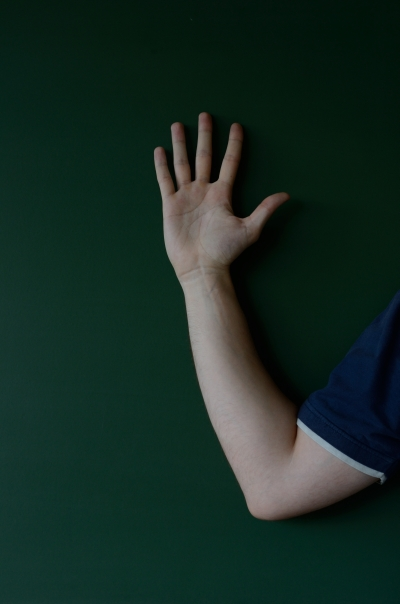
\includegraphics[width=\textwidth]{images/results/cross/5_A_hgr2B_id10_1_ecu_hgr_x.jpg}
     \end{subfigure}
     \hfill
     \begin{subfigure}[b]{0.23\textwidth}
         \centering
         
\includegraphics[width=\textwidth]{images/results/cross/5_A_hgr2B_id10_1_ecu_hgr_y.png}
     \end{subfigure}
    \hfill
     \begin{subfigure}[b]{0.23\textwidth}
         \centering
         
\includegraphics[width=\textwidth]{images/results/cross/5_A_hgr2B_id10_1_ecu_hgr_skinny_123.png}
     \end{subfigure}
    \hfill
     \begin{subfigure}[b]{0.23\textwidth}
         \centering
         
\includegraphics[width=\textwidth]{images/results/cross/5_A_hgr2B_id10_1_ecu_hgr_bayes.png}
     \end{subfigure}}
     
     \resizebox{0.8\textwidth}{0.17\textheight}{
     % ROW 2
     \begin{subfigure}[b]{0.23\textwidth}
         \centering
         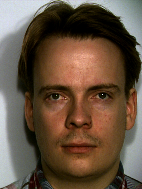
\includegraphics[width=\textwidth]{images/results/cross/aa46_1.color.d3_ecu_sch_x.png}
     \end{subfigure}
     \hfill
     \begin{subfigure}[b]{0.23\textwidth}
         \centering
         
\includegraphics[width=\textwidth]{images/results/cross/aa46_1.color.d3_ecu_sch_y.png}
     \end{subfigure}
    \hfill
     \begin{subfigure}[b]{0.23\textwidth}
         \centering
         
\includegraphics[width=\textwidth]{images/results/cross/aa46_1.color.d3_ecu_sch_skinny283.png}
     \end{subfigure}
    \hfill
     \begin{subfigure}[b]{0.23\textwidth}
         \centering
         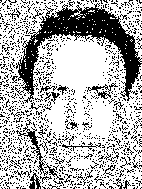
\includegraphics[width=\textwidth]{images/results/cross/aa46_1.color.d3_ecu_sch_bayes.png}
     \end{subfigure}}
    
     \resizebox{0.8\textwidth}{0.18\textheight}{
     % ROW 3
     \begin{subfigure}[b]{0.23\textwidth}
         \centering
         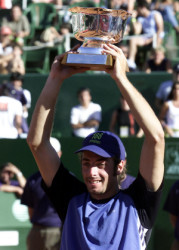
\includegraphics[width=\textwidth]{images/results/cross/att-massu.jpg_ecu_sch_x.png}
     \end{subfigure}
     \hfill
     \begin{subfigure}[b]{0.23\textwidth}
         \centering
         
\includegraphics[width=\textwidth]{images/results/cross/att-massu_ecu_sch_y.png}
     \end{subfigure}
    \hfill
     \begin{subfigure}[b]{0.23\textwidth}
         \centering
         
\includegraphics[width=\textwidth]{images/results/cross/att-massu.jpg_ecu_sch_skinny_157.png}
     \end{subfigure}
    \hfill
     \begin{subfigure}[b]{0.23\textwidth}
         \centering
         
\includegraphics[width=\textwidth]{images/results/cross/att-massu_ecu_sch_bayes.png}
     \end{subfigure}}
     
     \resizebox{0.8\textwidth}{0.08\textheight}{
     % ROW 4
     \begin{subfigure}[b]{0.23\textwidth}
         \centering
         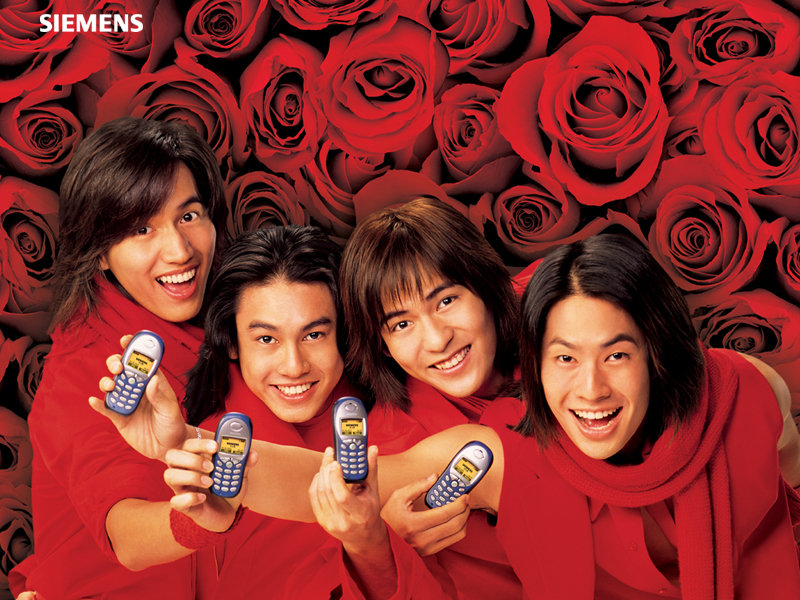
\includegraphics[width=\textwidth]{images/results/cross/im00593_sch_ecu_x.jpg}
     \end{subfigure}
     \hfill
     \begin{subfigure}[b]{0.23\textwidth}
         \centering
         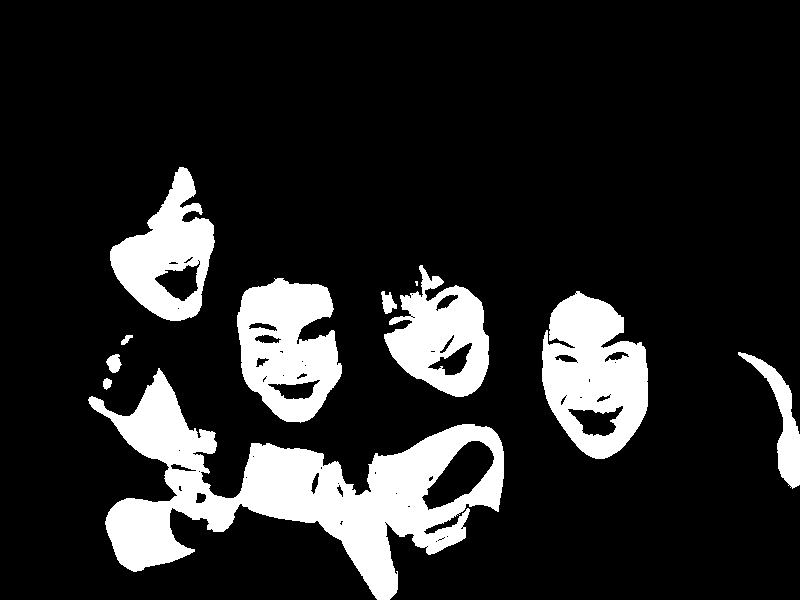
\includegraphics[width=\textwidth]{images/results/cross/im00593_sch_ecu_y.png}
     \end{subfigure}
    \hfill
     \begin{subfigure}[b]{0.23\textwidth}
         \centering
         \includegraphics[width=\textwidth]{images/results/cross/im00593_sch_ecu_skinny_424.png}
     \end{subfigure}
    \hfill
     \begin{subfigure}[b]{0.23\textwidth}
         \centering
         \includegraphics[width=\textwidth]{images/results/cross/im00593_sch_ecu_bayes.png}
     \end{subfigure}}
     
     \resizebox{0.8\textwidth}{0.2\textheight}{
     % ROW 5
     \begin{subfigure}[b]{0.23\textwidth}
         \centering
         \includegraphics[width=\textwidth]{images/results/cross/linda_rgb_hgr_sch_x.png}
     \end{subfigure}
     \hfill
     \begin{subfigure}[b]{0.23\textwidth}
         \centering
         \includegraphics[width=\textwidth]{images/results/cross/linda_rgb_hgr_sch_y.png}
     \end{subfigure}
    \hfill
     \begin{subfigure}[b]{0.23\textwidth}
         \centering
         \includegraphics[width=\textwidth]{images/results/cross/linda_rgb_hgr_sch_skinny120.png}
     \end{subfigure}
    \hfill
     \begin{subfigure}[b]{0.23\textwidth}
         \centering
         \includegraphics[width=\textwidth]{images/results/cross/linda_rgb_hgr_sch_bayes.png}
     \end{subfigure}}
     
     \resizebox{0.8\textwidth}{0.10\textheight}{
     % ROW 6
     \begin{subfigure}[b]{0.23\textwidth}
         \centering
         \includegraphics[width=\textwidth]{images/results/cross/w-020-7.color.d3_hgr_sch_x.png}
         \caption{}
     \end{subfigure}
     \hfill
     \begin{subfigure}[b]{0.23\textwidth}
         \centering
         \includegraphics[width=\textwidth]{images/results/cross/w-020-7.color.d3_hgr_sch_y.png}
         \caption{}
     \end{subfigure}
    \hfill
     \begin{subfigure}[b]{0.23\textwidth}
         \centering
         \includegraphics[width=\textwidth]{images/results/cross/w-020-7.color.d3_hgr_sch_skinny_426.png}
         \caption{}
     \end{subfigure}
    \hfill
     \hfill
     \begin{subfigure}[b]{0.23\textwidth}
         \centering
         \includegraphics[width=\textwidth]{images/results/cross/w-020-7.color.d3_hgr_sch_bayes.png}
         \caption{}
     \end{subfigure}}
\caption{Skin detection results in datasets cross evaluation: (a) the input image; (b) the ground truth; (c) Tarasiewicz \textit{et al.} 2020~\cite{tarasiewicz2020skinny}; (d) Acharjee~\cite{acharjee2018skin}}
\label{fig:cross-normal-samples}
\end{figure}%


\FloatBarrier
%%%%%%%%%%%%%%%%%%%%%%%%%%%%%%%%%%%%%%%%%%%%%%%%%%%%%%%%%%%%%%%%%%%%%%%%
\section{Performance on single Skin tones}
%%%%%%%%%%%%%%%%%%%%%%%%%%%%%%%%%%%%%%%%%%%%%%%%%%%%%%%%%%%%%%%%%%%%%%%%

In the single evaluation of the skin tones sub-datasets (present at \autoref{tab:base-skin-tones}), the U-Net outperforms the competitors in all cases, and the thresholding approach comes last in all cases.
The learning approaches describe a very low standard deviation on the darker skin tones, indicating that the diversity of the images might not be very high.
Tarasiewicz \textit{et al.} 2020~\cite{tarasiewicz2020skinny} reports outstanding scores, having almost ground truth-like predictions, as described by the D\textsubscript{prs} measure.
Brancati \textit{et al.} 2017~\cite{brancati2017human} instead describes horrible results, which may indicate that the skin clustering rules are leaving out the darker skin pixels.
The machine learning methods have the highest difficulty at classifying the medium skin tones, which pictures include a lot of difficult scenarios, such as clay terrains that are skin-like colored.
Despite the troubles, all the approaches report generally good scores on both medium and light skin tones, especially the machine learning methods.

\begin{table}[ht]
    \centering
    \resizebox{\columnwidth}{!}{
    \begin{tabular}{clccc}
    \toprule
    & Method\textbackslash Database & DARK & MEDIUM & LIGHT \\
    \midrule
    %
    %
    \multirow{3}{*}{{$F_1 \uparrow$}}
        & Tarasiewicz \textit{et al.}~\cite{tarasiewicz2020skinny}
        & $\pmb{0.9529 \pm 0.00}$ & $\pmb{0.9260 \pm 0.15}$ & $\pmb{0.9387 \pm 0.12}$ \\
        %
        & Acharjee~\cite{acharjee2018skin}
        & $\underline{0.8123 \pm 0.02}$ & $\underline{0.7634 \pm 0.19}$ & $\underline{0.8001 \pm 0.15}$ \\
        %
        & Brancati \textit{et al.}~\cite{brancati2017human}
        & $0.2620 \pm 0.14$ & $0.6316 \pm 0.20$ & $0.6705 \pm 0.14$ \\[5pt]
        %
        %
    \multirow{3}{*}{{$IoU \uparrow$}}
        & Tarasiewicz \textit{et al.}~\cite{tarasiewicz2020skinny}
        & $\pmb{0.9100 \pm 0.01}$ & $\pmb{0.8883 \pm 0.18}$ & $\pmb{0.9006 \pm 0.14}$ \\
        %
        & Acharjee~\cite{acharjee2018skin}
        & $\underline{0.6844 \pm 0.03}$ & $\underline{0.6432 \pm 0.17}$ & $\underline{0.6870 \pm 0.16}$ \\
        %
        & Brancati \textit{et al.}~\cite{brancati2017human}
        & $0.1587 \pm 0.10$ & $0.4889 \pm 0.19$ & $0.5190 \pm 0.14$ \\[5pt]
        %
        %
    \multirow{3}{*}{{$D_{prs} \downarrow$}}
        & Tarasiewicz \textit{et al.}~\cite{tarasiewicz2020skinny}
        & $\pmb{0.0720 \pm 0.01}$ & $\pmb{0.1078 \pm 0.21}$ & $\pmb{0.0926 \pm 0.15}$ \\
        %
        & Acharjee~\cite{acharjee2018skin}
        & $\underline{0.3406 \pm 0.05}$ & $\underline{0.3452 \pm 0.23}$ & $\underline{0.3054 \pm 0.20}$ \\
        %
        & Brancati \textit{et al.}~\cite{brancati2017human}
        & $0.8548 \pm 0.12 $ & $0.5155 \pm 0.24$ & $0.4787 \pm 0.17$\\
        %
        %
    \bottomrule
    \end{tabular}}
    \caption{Single evaluation on skin tones.\\
     For each dataset: methods are eventually trained on the training set, in the case of trainable methods, and then predictions are performed on the test set.\\
     For example, with DARK as the dataset, it means that a method is trained using the training set of DARK, if the method is trainable, and then tested on the test set of DARK.
    }
    \label{tab:base-skin-tones}
\end{table}

Some interesting instances can be seen in \autoref{fig:base-skintones-samples}.
The first two rows depict darker skin tones.
In both examples, it is possible to notice a pattern in the classification of each approach: Tarasiewicz \textit{et al.} 2020~\cite{tarasiewicz2020skinny} produces almost ground truth-like predictions; the statistical method tends to exaggerate on classifying skin pixels, but has an excellent number of True Positives; Brancati \textit{et al.} 2017~\cite{brancati2017human} seems to fail at classifying the darkest skin tones.
The next two rows represent medium skin tones.
The following row reports similar results to the dark skin tones rows, but in this case the thresholding approach has good results.
It is noticeable that, while the statistical method tends to include many False Positives, the thresholding one is a lot more conservative, marking only the inner regions of the face, which are sufficient for describing the face shape.
The last row of medium skin tones represents a tricky background with a clay terrain.
Tarasiewicz \textit{et al.} 2020~\cite{tarasiewicz2020skinny} produces a very good prediction, while the other approaches include many False Positives.
Acharjee 2018~\cite{acharjee2018skin} reports a tremendous number of False Positives, while Brancati \textit{et al.} 2017~\cite{brancati2017human} is deceived by the clay terrain and ruins its otherwise excellent classification.
The last two rows feature people with light skin tones.
In the starting row, the U-Net and the rule-based approaches have very good predictions, with Tarasiewicz \textit{et al.} 2020~\cite{tarasiewicz2020skinny} incorporating more False Positives, and Brancati \textit{et al.} 2017~\cite{brancati2017human} including more False Negatives.
The statistical approach reports once again a huge number of False Positives.
The last row depicts good results on all methods and shows some limitations that Brancati \textit{et al.} 2017~\cite{brancati2017human} seems to have on tricky lighting conditions.

\begin{figure}[h]
     \centering
     % ROW 1
     \begin{subfigure}[b]{0.18\textwidth}
         \centering
         \includegraphics[width=\textwidth]{images/results/base_st/dd109.color.d3_x.png}
     \end{subfigure}
     \hfill
     \begin{subfigure}[b]{0.18\textwidth}
         \centering
         \includegraphics[width=\textwidth]{images/results/base_st/dd109.color.d3_y.png}
     \end{subfigure}
    \hfill
     \begin{subfigure}[b]{0.18\textwidth}
         \centering
         \includegraphics[width=\textwidth]{images/results/base_st/dd109.color.d3_skinny_4.png}
     \end{subfigure}
    \hfill
     \begin{subfigure}[b]{0.18\textwidth}
         \centering
         \includegraphics[width=\textwidth]{images/results/base_st/dd109.color.d3_bayes.png}
     \end{subfigure}
    \hfill
     \begin{subfigure}[b]{0.18\textwidth}
         \centering
         \includegraphics[width=\textwidth]{images/results/base_st/dd109.color.d3_dyc.png}
     \end{subfigure}
     % ROW 2
     \begin{subfigure}[b]{0.18\textwidth}
         \centering
         \includegraphics[width=\textwidth]{images/results/base_st/dd110.color.d3_x.png}
     \end{subfigure}
     \hfill
     \begin{subfigure}[b]{0.18\textwidth}
         \centering
         \includegraphics[width=\textwidth]{images/results/base_st/dd110.color.d3_y.png}
     \end{subfigure}
    \hfill
     \begin{subfigure}[b]{0.18\textwidth}
         \centering
         \includegraphics[width=\textwidth]{images/results/base_st/dd110.color.d3_skinny_2.png}
     \end{subfigure}
    \hfill
     \begin{subfigure}[b]{0.18\textwidth}
         \centering
         \includegraphics[width=\textwidth]{images/results/base_st/dd110.color.d3_bayes.png}
     \end{subfigure}
     \hfill
     \begin{subfigure}[b]{0.18\textwidth}
         \centering
         \includegraphics[width=\textwidth]{images/results/base_st/dd110.color.d3_dyc.png}
     \end{subfigure}
     % ROW 3
     \begin{subfigure}[b]{0.18\textwidth}
         \centering
         \includegraphics[width=\textwidth]{images/results/base_st/dd121.color.d3_x.png}
     \end{subfigure}
     \hfill
     \begin{subfigure}[b]{0.18\textwidth}
         \centering
         \includegraphics[width=\textwidth]{images/results/base_st/dd121.color.d3_y.png}
     \end{subfigure}
    \hfill
     \begin{subfigure}[b]{0.18\textwidth}
         \centering
         \includegraphics[width=\textwidth]{images/results/base_st/dd121.color.d3_skinny_13.png}
     \end{subfigure}
    \hfill
     \begin{subfigure}[b]{0.18\textwidth}
         \centering
         \includegraphics[width=\textwidth]{images/results/base_st/dd121.color.d3_bayes.png}
     \end{subfigure}
    \hfill
     \begin{subfigure}[b]{0.18\textwidth}
         \centering
         \includegraphics[width=\textwidth]{images/results/base_st/dd121.color.d3_dyc.png}
     \end{subfigure}
     % ROW 4
     \begin{subfigure}[b]{0.18\textwidth}
         \centering
         \includegraphics[width=\textwidth]{images/results/base_st/ivan1_x.png}
     \end{subfigure}
     \hfill
     \begin{subfigure}[b]{0.18\textwidth}
         \centering
         \includegraphics[width=\textwidth]{images/results/base_st/ivan1_y.png}
     \end{subfigure}
    \hfill
     \begin{subfigure}[b]{0.18\textwidth}
         \centering
         \includegraphics[width=\textwidth]{images/results/base_st/ivan1_skinny_2.png}
     \end{subfigure}
    \hfill
     \begin{subfigure}[b]{0.18\textwidth}
         \centering
         \includegraphics[width=\textwidth]{images/results/base_st/ivan1_bayes.png}
     \end{subfigure}
    \hfill
     \begin{subfigure}[b]{0.18\textwidth}
         \centering
         \includegraphics[width=\textwidth]{images/results/base_st/ivan1_dyc.png}
     \end{subfigure}
     % ROW 5
     \begin{subfigure}[b]{0.18\textwidth}
         \centering
         \includegraphics[width=\textwidth]{images/results/base_st/wd2002-sue-shaded-hat_x.png}
     \end{subfigure}
     \hfill
     \begin{subfigure}[b]{0.18\textwidth}
         \centering
         \includegraphics[width=\textwidth]{images/results/base_st/wd2002-sue-shaded-hat_y.png}
     \end{subfigure}
    \hfill
     \begin{subfigure}[b]{0.18\textwidth}
         \centering
         \includegraphics[width=\textwidth]{images/results/base_st/wd2002-sue-shaded-hat_skinny_22.png}
     \end{subfigure}
    \hfill
     \begin{subfigure}[b]{0.18\textwidth}
         \centering
         \includegraphics[width=\textwidth]{images/results/base_st/wd2002-sue-shaded-hat_bayes.png}
     \end{subfigure}
    \hfill
     \begin{subfigure}[b]{0.18\textwidth}
         \centering
         \includegraphics[width=\textwidth]{images/results/base_st/wd2002-sue-shaded-hat_dyc.png}
     \end{subfigure}
     % ROW 6
     \begin{subfigure}[b]{0.18\textwidth}
         \centering
         \includegraphics[width=\textwidth]{images/results/base_st/m-022-5.color.d3_x.png}
         \caption{}
     \end{subfigure}
     \hfill
     \begin{subfigure}[b]{0.18\textwidth}
         \centering
         \includegraphics[width=\textwidth]{images/results/base_st/m-022-5.color.d3_y.png}
         \caption{}
     \end{subfigure}
    \hfill
     \begin{subfigure}[b]{0.18\textwidth}
         \centering
         \includegraphics[width=\textwidth]{images/results/base_st/m-022-5.color.d3_skinny_25.png}
         \caption{}
     \end{subfigure}
    \hfill
     \begin{subfigure}[b]{0.18\textwidth}
         \centering
         \includegraphics[width=\textwidth]{images/results/base_st/m-022-5.color.d3_bayes.png}
         \caption{}
     \end{subfigure}
     \hfill
     \begin{subfigure}[b]{0.18\textwidth}
         \centering
         \includegraphics[width=\textwidth]{images/results/base_st/m-022-5.color.d3_dyc.png}
         \caption{}
     \end{subfigure}
        \caption{Skin detection results in skin tones single evaluation: (a) the input image; (b) the ground truth; (c) Tarasiewicz \textit{et al.} 2020~\cite{tarasiewicz2020skinny}; (d) Acharjee~\cite{acharjee2018skin}; (e) Brancati \textit{et al.} 2017~\cite{brancati2017human}.}
        \label{fig:base-skintones-samples}
\end{figure}


\FloatBarrier
%%%%%%%%%%%%%%%%%%%%%%%%%%%%%%%%%%%%%%%%%%%%%%%%%%%%%%%%%%%%%%%%%%%%%%%%
\section{Performance across Skin tones}
%%%%%%%%%%%%%%%%%%%%%%%%%%%%%%%%%%%%%%%%%%%%%%%%%%%%%%%%%%%%%%%%%%%%%%%%

The cross evaluation of the skin tones sub-datasets, \autoref{tab:cross-skin-tones}), describes some interesting situations.
As usual, the U-Net outperforms the other machine learning approach in most situations, but it is outperformed a pair of times.
In fact, using the darker skin tones as training and predicting on the medium skin tones makes Acharjee 2018~\cite{acharjee2018skin} the seemingly better classifier.
It describes best scores in all metrics but the difference between F\textsubscript{1} and D\textsubscript{prs}, with also a lower population standard deviation.
The dark sub-dataset was the smallest one and therefore has been data-augmented.
However, the augmentation has been performed with light transformations that do not detach from the original images too much.
Hence, these scores may indicate that Acharjee 2018~\cite{acharjee2018skin} performs better with a smaller training set.
Anyway, Tarasiewicz \textit{et al.} 2020~\cite{tarasiewicz2020skinny} describes only slightly worse results and reports good classifications in this scenario too.
The higher difference between F\textsubscript{1} and D\textsubscript{prs} may indicate the usual greedy that the statistical method demonstrates on False Positives.
The dark on light case is particularly interesting because the statistical approach wins on the F\textsubscript{1}-Score, but is outperformed in all the others.
Winning on the F\textsubscript{1}-Score and losing on the IoU means that the statistical approach picks more True Positives than the deep learning one.
Tarasiewicz \textit{et al.} 2020~\cite{tarasiewicz2020skinny} also describes more unstable results as the population standard deviation is higher.
The F\textsubscript{1} and IoU scores are relatively close between the approaches, but the D\textsubscript{prs} is far better with Tarasiewicz \textit{et al.} 2020~\cite{tarasiewicz2020skinny}.
This behavior may suggest, along with the F\textsubscript{1} and IoU considerations, and the fact that their difference is higher on the statistical method, the presence of many False Positives and/or False Negatives, which however seems unlikely given the previous observations, on the statistical method predictions.
All the other situations have the U-Net winning on the scores by a great degree.
In the medium on dark situation, Acharjee 2018~\cite{acharjee2018skin} describes a very high D\textsubscript{prs}, even higher than the light on dark case, where the F\textsubscript{1} and IoU scores are worse.
This is a clear indicator that the Specificity is driving the prediction away from the ideal ground truth, so it may be an indicator of a very small number of True Negatives.
Tarasiewicz \textit{et al.} 2020~\cite{tarasiewicz2020skinny} presents the highest score in the light on medium case, which may be a signal of the need of having bigger training data, but on the other hand, it performs far worse on the light on dark case, indicating that a bigger training data might not be sufficient.
In fact, the U-Net describes the best average score by training on the medium skin tones, which represent a smaller dataset than the lighter skin tones, but a midpoint between the colors of darker and lighter skin tones.
This may be a representation of how the Neural Network adapts and learns to classify new skin tones.

Some interesting instances are reported in \autoref{fig:cross-skintones-samples}.
The first two rows represent dark on medium cases.
The results seem to confirm the earlier guesses on the statistical method incorporating a lot of False Positives.
Tarasiewicz \textit{et al.} 2020~\cite{tarasiewicz2020skinny} depicts a terrible classification, with a lot of False Positives and False Negatives.
In the second row, the tricky lighting causes troubles to the U-Net, which provides another terrible prediction, while the statistical method has a far better prediction, despite including a lot of False Positives too.
The third row and the fourth row represent dark on light situations.
Tarasiewicz \textit{et al.} 2020~\cite{tarasiewicz2020skinny} produces an awful prediction even in these cases, featuring particularly a lot of False Negatives.
Acharjee 2018~\cite{acharjee2018skin} does the opposite and once again exaggerates as usual with the classification of skin pixels.
The original images of these two rows are also featured in \autoref{fig:cross-normal-samples}, where they reported similar issues, so it seems that both approaches struggle to adapt to skin pixels different from the ones of the training set in these types of images.
The smallest image depicts a quite extreme and unnatural level of lighting, hence the issues are easily justifiable.
The other image seems to depict a more natural skin tone, but it must be taken into account that it may still be far from the skin tones of the training set, which may be too light or dark. 
The fifth row features a medium on dark case, where the hypothesis of having very few True Negatives, driving the D\textsubscript{prs} measure high, seems confirmed.
Tarasiewicz \textit{et al.} 2020~\cite{tarasiewicz2020skinny} on the other hand performs a quite good classification, marking almost correctly most of the skin regions.
The last row represents a light on dark case on the same original picture of the previous row, with the purpose of a quick comparison.
In this case, the statistical approach does a much better job, especially at predicting non-skin pixels, which may indicate that the light sub-dataset contains more images featuring sky and water labeled as non-skin pixels.
Tarasiewicz \textit{et al.} 2020~\cite{tarasiewicz2020skinny} performs quite similarly to the previous instance.

\begin{table}[ht]
    \centering
    \resizebox{\columnwidth}{!}{
    \begin{tabular}{clcccccc}
    \toprule
    \multicolumn{1}{c}{} & \multicolumn{1}{c}{Training} 
    & \multicolumn{2}{c}{DARK} & \multicolumn{2}{c}{MEDIUM} & \multicolumn{2}{c}{LIGHT} \\\multicolumn{1}{c}{} & \multicolumn{1}{c}{Testing}  & \multicolumn{1}{c}{MEDIUM}  & \multicolumn{1}{c}{LIGHT}  & \multicolumn{1}{c}{DARK}  & \multicolumn{1}{c}{LIGHT}  & \multicolumn{1}{c}{DARK}  & \multicolumn{1}{c}{MEDIUM} \\\midrule\multirow{2}{*}{{$F_1$ $\uparrow$}}& Taras. \textit{et al.}~\cite{tarasiewicz2020skinny}\rule{0pt}{14pt} & \monosp{0.7300 \pm 0.25} & \monosp{0.7262 \pm 0.26} & \monosp{\monobold{0.8447 \pm 0.13}} & \monosp{\monobold{0.8904 \pm 0.14}} & \monosp{\monobold{0.7660 \pm 0.17}} & \monosp{\monobold{0.9229 \pm 0.11}}\\& Acharjee~\cite{acharjee2018skin} & \monosp{\monobold{0.7928 \pm 0.11}} & \monosp{\monobold{0.7577 \pm 0.12}} & \monosp{0.5628 \pm 0.14} & \monosp{0.7032 \pm 0.14} & \monosp{0.5293 \pm 0.20} & \monosp{0.7853 \pm 0.11}\\\multirow{2}{*}{{$IoU$ $\uparrow$}}& Taras. \textit{et al.}~\cite{tarasiewicz2020skinny}\rule{0pt}{14pt} & \monosp{0.6279 \pm 0.27} & \monosp{\monobold{0.6276 \pm 0.28}} & \monosp{\monobold{0.7486 \pm 0.15}} & \monosp{\monobold{0.8214 \pm 0.16}} & \monosp{\monobold{0.6496 \pm 0.21}} & \monosp{\monobold{0.8705 \pm 0.13}}\\& Acharjee~\cite{acharjee2018skin} & \monosp{\monobold{0.6668 \pm 0.11}} & \monosp{0.6229 \pm 0.13} & \monosp{0.4042 \pm 0.13} & \monosp{0.5571 \pm 0.14} & \monosp{0.3852 \pm 0.19} & \monosp{0.6574 \pm 0.12}\\\multirow{2}{*}{{$D_{prs}$ $\downarrow$}}& Taras. \textit{et al.}~\cite{tarasiewicz2020skinny}\rule{0pt}{14pt} & \monosp{0.3805 \pm 0.33} & \monosp{\monobold{0.3934 \pm 0.34}} & \monosp{\monobold{0.2326 \pm 0.17}} & \monosp{\monobold{0.1692 \pm 0.18}} & \monosp{\monobold{0.3402 \pm 0.21}} & \monosp{\monobold{0.1192 \pm 0.16}}\\& Acharjee~\cite{acharjee2018skin} & \monosp{\monobold{0.3481 \pm 0.16}} & \monosp{0.4679 \pm 0.18} & \monosp{0.6802 \pm 0.20} & \monosp{0.5376 \pm 0.23} & \monosp{0.6361 \pm 0.22} & \monosp{0.3199 \pm 0.16}\\\multirow{2}{*}{{$F_1 - IoU$ $\downarrow$}}& Taras. \textit{et al.}~\cite{tarasiewicz2020skinny}\rule{0pt}{14pt} & \monosp{\monobold{0.1021}} & \monosp{\monobold{0.0986}} & \monosp{\monobold{0.0961}} & \monosp{\monobold{0.0690}} & \monosp{\monobold{0.1164}} & \monosp{\monobold{0.0524}}\\& Acharjee~\cite{acharjee2018skin} & \monosp{0.1260} & \monosp{0.1348} & \monosp{0.1586} & \monosp{0.1461} & \monosp{0.1441} & \monosp{0.1279}\\
    \bottomrule
    \end{tabular}}
    \caption{Cross evaluation on skin tones.\\
        For each dataset: methods are trained on the training set and then predictions are performed on all the images of every other datasets.\\
        For example, with DARK as the training dataset and LIGHT as the testing dataset, it means that a method is trained using the training set of DARK, and then tested on all the LIGHT dataset.}
    \label{tab:cross-skin-tones}
\end{table}

\begin{figure}[h]
     \centering
     
     \resizebox{0.8\textwidth}{0.17\textheight}{
     % ROW 1
     \begin{subfigure}[b]{0.23\textwidth}
         \centering
         \includegraphics[width=\textwidth]{images/results/cross_st/clay_dark_med_x.png}
     \end{subfigure}
     \hfill
     \begin{subfigure}[b]{0.23\textwidth}
         \centering
         \includegraphics[width=\textwidth]{images/results/cross_st/clay_dark_med_y.png}
     \end{subfigure}
    \hfill
     \begin{subfigure}[b]{0.23\textwidth}
         \centering
         \includegraphics[width=\textwidth]{images/results/cross_st/clay_dark_med_skinny_92.png}
     \end{subfigure}
    \hfill
     \begin{subfigure}[b]{0.23\textwidth}
         \centering
         \includegraphics[width=\textwidth]{images/results/cross_st/clay_dark_med_bayes.png}
     \end{subfigure}}
     
    \resizebox{0.8\textwidth}{0.08\textheight}{
     % ROW 2
     \begin{subfigure}[b]{0.23\textwidth}
         \centering
         \includegraphics[width=\textwidth]{images/results/cross_st/w-020-7.color.d3_dark_med_x.png}
     \end{subfigure}
     \hfill
     \begin{subfigure}[b]{0.23\textwidth}
         \centering
         \includegraphics[width=\textwidth]{images/results/cross_st/w-020-7.color.d3.png}
     \end{subfigure}
    \hfill
     \begin{subfigure}[b]{0.23\textwidth}
         \centering
         \includegraphics[width=\textwidth]{images/results/cross_st/w-020-7.color.d3_dark_med_skinny_57.png}
     \end{subfigure}
    \hfill
     \begin{subfigure}[b]{0.23\textwidth}
         \centering
         \includegraphics[width=\textwidth]{images/results/cross_st/w-020-7.color.d3_dark_med_bayes.png}
     \end{subfigure}}
     
    \resizebox{0.8\textwidth}{0.20\textheight}{
     % ROW 3
     \begin{subfigure}[b]{0.23\textwidth}
         \centering
         \includegraphics[width=\textwidth]{images/results/cross_st/linda_rgb_dark_light_x.png}
     \end{subfigure}
     \hfill
     \begin{subfigure}[b]{0.23\textwidth}
         \centering
         \includegraphics[width=\textwidth]{images/results/cross_st/linda_rgb_dark_light_y.png}
     \end{subfigure}
    \hfill
     \begin{subfigure}[b]{0.23\textwidth}
         \centering
         \includegraphics[width=\textwidth]{images/results/cross_st/linda_rgb_dark_light_skinny_293.png}
     \end{subfigure}
    \hfill
     \begin{subfigure}[b]{0.23\textwidth}
         \centering
         \includegraphics[width=\textwidth]{images/results/cross_st/linda_rgb_dark_light_bayes.png}
     \end{subfigure}}
     
    \resizebox{0.8\textwidth}{0.07\textheight}{
     % ROW 4
     \begin{subfigure}[b]{0.23\textwidth}
         \centering
         \includegraphics[width=\textwidth]{images/results/cross_st/outdoor_cooking_dark_light_x.png}
     \end{subfigure}
     \hfill
     \begin{subfigure}[b]{0.23\textwidth}
         \centering
         \includegraphics[width=\textwidth]{images/results/cross_st/outdoor_cooking_dark_light_y.png}
     \end{subfigure}
    \hfill
     \begin{subfigure}[b]{0.23\textwidth}
         \centering
         \includegraphics[width=\textwidth]{images/results/cross_st/outdoor_cooking_dark_light_skinny_3.png}
     \end{subfigure}
    \hfill
     \begin{subfigure}[b]{0.23\textwidth}
         \centering
         \includegraphics[width=\textwidth]{images/results/cross_st/outdoor_cooking_dark_light_bayes.png}
     \end{subfigure}}
     
     \resizebox{0.8\textwidth}{0.18\textheight}{
     % ROW 5
     \begin{subfigure}[b]{0.23\textwidth}
         \centering
         \includegraphics[width=\textwidth]{images/results/cross_st/mike_med_dark_x.png}
     \end{subfigure}
     \hfill
     \begin{subfigure}[b]{0.23\textwidth}
         \centering
         \includegraphics[width=\textwidth]{images/results/cross_st/mike_med_dark_y.png}
     \end{subfigure}
    \hfill
     \begin{subfigure}[b]{0.23\textwidth}
         \centering
         \includegraphics[width=\textwidth]{images/results/cross_st/mike_med_dark_skinny_19.png}
     \end{subfigure}
    \hfill
     \begin{subfigure}[b]{0.23\textwidth}
         \centering
         \includegraphics[width=\textwidth]{images/results/cross_st/mike_med_dark_bayes.png}
     \end{subfigure}}
     
     \resizebox{0.8\textwidth}{0.20\textheight}{
     % ROW 6
     \begin{subfigure}[b]{0.23\textwidth}
         \centering
         \includegraphics[width=\textwidth]{images/results/cross_st/mike_light_dark_x.png}
         \caption{}
     \end{subfigure}
     \hfill
     \begin{subfigure}[b]{0.23\textwidth}
         \centering
         \includegraphics[width=\textwidth]{images/results/cross_st/mike_light_dark_y.png}
         \caption{}
     \end{subfigure}
    \hfill
     \begin{subfigure}[b]{0.23\textwidth}
         \centering
         \includegraphics[width=\textwidth]{images/results/cross_st/mike_light_dark_skinny_24.png}
         \caption{}
     \end{subfigure}
    \hfill
     \hfill
     \begin{subfigure}[b]{0.23\textwidth}
         \centering
         \includegraphics[width=\textwidth]{images/results/cross_st/mike_light_dark_bayes.png}
         \caption{}
     \end{subfigure}}
\caption{Skin detection results in skin tones cross evaluation: (a) the input image; (b) the ground truth; (c) Tarasiewicz \textit{et al.} 2020~\cite{tarasiewicz2020skinny}; (d) Acharjee~\cite{acharjee2018skin}.}
\label{fig:cross-skintones-samples}
\end{figure}%


\FloatBarrier
%%%%%%%%%%%%%%%%%%%%%%%%%%%%%%%%%%%%%%%%%%%%%%%%%%%%%%%%%%%%%%%%%%%%%%%%
\section{Inference time}
%%%%%%%%%%%%%%%%%%%%%%%%%%%%%%%%%%%%%%%%%%%%%%%%%%%%%%%%%%%%%%%%%%%%%%%%

The inference time evaluation follows these rules:
\begin{itemize}
    \item Image loading into memory is excluded.
    \item Image saving to disk is excluded.
    \item The measurement starts when the algorithm starts.
    \item Pre-processing and post-processing, if present, are included in the measured execution time.
\end{itemize}
It has been defined a set of 14 images of the same dimensions to use as the performance evaluation set: it is composed of the first 14 images of the ECU dataset of size $352\times288$.
One image at a time has been processed by the methods and the resulting execution time has been saved.
The set of pictures has been processed 5 times and, each time, the average measurement time has been calculated.
Finally, the five average values have been averaged into a single value and the standard deviation has been computed.\\
% SYSTEM
The inference time measurements have all been performed on an i7 4770k processor running on Pop!\_OS 20.10 x86\_64 with 16 GB of RAM.
The rule-based~\cite{brancati2017human} method uses OpenCV 2.4.9 and is compiled with g++ version 10.2.0-13ubuntu1.
The other methods use Python 3.8.6 64bit. Tarasiewicz \textit{et al.} 2020~\cite{tarasiewicz2020skinny} uses Tensorflow 2.5.0 for inference time measurements, but the models has been trained using Google Colab with Tensorflow 2.4.1 and Python 3.7.10.

The inference time evaluation (found in \autoref{tab:inference-performance}) reports a very simple situation.
The thresholding approach is much faster than the other approaches and also expresses a null standard deviation, which highlights the impartiality that the algorithm describes with respect to images of different content.
The statistical approach comes second and reports a really low standard deviation score too.
Despite coming second, its score is far away from the first place.
At the last place lies Tarasiewicz \textit{et al.} 2020~\cite{tarasiewicz2020skinny}, with a score of almost one second per image and the biggest standard deviation score, which may indicate that its inference times depend slightly on the pixels of an image.
%Probably on a GPU Skinny would have scored differently.
The scores indicate that the only suitable approach to real-time skin detection on a CPU may be Brancati \textit{et al.} 2017~\cite{brancati2017human}, which is very fast and could describe the same behavior on less powerful hardware.

\begin{table}[ht]
    \centering
    %\resizebox{\columnwidth}{!}{
        \begin{tabular}{lc}
        \toprule
        & Inference time (seconds)\\
        \midrule
        Tarasiewicz \textit{et al.}~\cite{tarasiewicz2020skinny} & \monosp{0.826581 \pm 0.043}\\
        Acharjee~\cite{acharjee2018skin} & \monosp{\underline{0.457534 \pm 0.002}}\\
        Brancati \textit{et al.}~\cite{brancati2017human} & \monosp{\monobold{0.007717 \pm 0.000}}\\
        \bottomrule
        \end{tabular}%}
    \caption{Inference time performance measurements.}
    \label{tab:inference-performance}
\end{table}
